% ch30-fp8-split-d-m4n2.tex — FP8(三)：split-D 与 M4N2——大 D 的两堵墙（RFC-K4）
% 源码：ffpa-attn(861d75e) cute/fp8/sm_120/split_d.cuh(956L) + split_d_m4n2.cuh(989L)
%       + attn_traits.cuh(L109-311) + softmax.cuh(L74-231) + dispatch/cute_fp8.cuh
\chapter{FP8（三）：split-D 与 M4N2——大 $D$ 的两堵墙}\label{ch:30}

\section{本章导读}

第~\ref{ch:29}~章的 persist-D 把整个 $K$ tile（$B_c\times D$）一次装进
smem、让单个 warp 独占 $O$ 的全部 $D$ 列。这在 $D\le 224$ 时是最优解；
但 $D$ 继续增大，会同时撞上\textbf{两堵墙}：

\begin{enumerate}[itemsep=0pt,topsep=2pt]
  \item \textbf{smem 墙}：$K$ tile 字节数 $O(D)$，99KB 预算装不下——
        由 \textbf{split-D}（D 维分块）解决；
  \item \textbf{寄存器墙}：$O$ 累加器 $O(D)$ 个 f32 寄存器/线程，逼近
        255 上限——由 \textbf{M4N2 TiledMMA}（atom 布局重排）解决。
\end{enumerate}

两堵墙正交：只做 split-D，寄存器照旧 $O(D)$；只做 M4N2，smem 照旧装不下。
ffpa-attn 的 dispatch 按 $D$ 三分（\texttt{dispatch/\allowbreak{}cute\_fp8.cuh}
L60--64）：

\begin{center}
\begin{tabular}{@{}llll@{}}
\toprule
$D$ 范围 & kernel & atom 布局 & $O$ 寄存器/线程 \\
\midrule
$D\le 224$ & \texttt{persist\_d}（第~\ref{ch:29}~章） & M8N1 & $D/2$ \\
$224<D<768$ & \texttt{split\_d.cuh}（本章） & M8N1 & $D/2$ \\
$D\ge 768$ & \texttt{split\_d\_m4n2.cuh}（本章） & M4N2 & $D/4$ \\
\bottomrule
\end{tabular}
\end{center}

本章先推导 split-D 的分块恒等式（为什么它是\textbf{精确}变换，一个比特
都不差），再建立 M4N2 的寄存器压力模型（为什么 $N$ 维劈开是数学上的唯一
出口），最后走读两个 kernel 的实现差异——特别是 M4N2 带来的多笔新代价：
P 的 SMEM roundtrip、跨 N-warp softmax 归约、$k_{Br}$ 减半与量化块
错位等。所有机制均以
fp8 家族为主线；fp16 家族同构（第~\ref{ch:25}~章已见其 fp16 版），fp4
家族见第~\ref{ch:32}~章。

\section{问题与动机}

\subsection{两堵墙的数量级}

smem 墙好算：fp8 下 1B/元素，$B_c=128$ 的 $K$ tile 在 $D=512$ 时是
64KB，加上 V stage 与 Q 就超 99KB 预算。persist-D 靠「K 槽位 0（Q 区）
复用给最后一个 K stage」
挤过去的前提是 $D\le 224$；$D$ 再大，唯一的路是把 $D$ 切块流水。

寄存器墙隐蔽一些。m16n8k32 atom 的 C-fragment 每 thread 持 4 个 f32；
M8N1 布局（8 个 M-warp、N 维单 warp 满编）下单 warp 独占输出的完整 $D$
列，$k_{Br}=128$ 时 $O$ 累加器寄存器数是
\begin{equation}\label{eq:30-oacc-m8n1}
O_{\text{acc}}=\frac{k_{Br}\cdot D}{256\ \text{threads}}=\frac{D}{2}
\quad(\text{f32 regs/thread},\ k_{Br}=128),
\end{equation}
$D=512$ 时 256 个寄存器\textbf{超出上限 1 个}（255）——边缘 spill；$D\ge 896$ 大量
spill 直接崩塌。实测（5090，fp16 家族同构）：$D=1024$ 时 M8N1 的
$O_{\text{acc}}=512$ regs 溢出到 local memory，吞吐掉到 $\sim$100T；
而 M4N2 同 $D$ 边缘 spill 仍有 154T。

\subsection{split-D 与 M4N2 各管一堵墙}

\textbf{split-D} 回答「smem 怎么装下」：把 $D$ 切成 $D/k_{VDChunk}$ 个
chunk，K/V 的 TMA 与 MMA 都按 chunk 流水，smem 只需常驻
$(k_{Br}+k_{Bc})\times k_{QKDChunk}+k_{Bc}\times k_{VDChunk}$ 每 stage，
与总 $D$ 无关。\textbf{M4N2} 回答「寄存器怎么装下」：把 atom 布局从
$(8,1,1)$ 换成 $(4,2,1)$——4 个 M-warp \textbf{乘} 2 个 N-warp——让每
thread 的 $O$ 列持有量减半（\ref{sec:30-regmodel}~节的推导）。

代价各自独立：split-D 多了每 chunk 一次 producer-consumer 握手；M4N2
使 $k_{Br}$ 从 128 减到 64（CTA 数翻倍）、P 必须走 SMEM roundtrip、
softmax 需要跨 N-warp 归约。交叉点在 $D=768$：之下 M8N1 更快（无
roundtrip 开销、$k_{Br}$ 大一倍），之上 M4N2 的寄存器红利开始统治
（30.6.2~节）。

\subsection{causal 精度的已知边界}

\texttt{split\_d.cuh} 的头注释（L40--43）声明了 causal 精度边界：
逐元素误差上界——causal 早期行 attend 的 key 少，
QK/P 量化误差无法被平均——
$O$ 误差可保持在 $10^{-1}$ 量级但 lse 误差可达 $\sim 6\times10^{-2}$
（近 1 概率的 e4m3 舍入），dense 则 $\sim 4\times10^{-3}$（m4n2 头注释无同款
声明，但精度结构相同）。本机实测
（30.6~节）三个 $D$ 的 causal 误差模式完全一致：序列前
$\sim$30\% 的行误差大、其余干净、dense 全绿——这是 fp8 路径的
\textbf{已知特性}而非 bug，工程解法是 hybrid（前若干行走 fp16
stage-1，\texttt{dispatch/cute\_fp8.cuh} L55--58 的 FC-3 注释），
不在本章展开。

\section{数学原理}

\subsection{split-D 分块恒等式：精确，不是近似}\label{sec:30-identity}

设 $D=\mathcal{D}_0\cup\mathcal{D}_1\cup\cdots$ 按 chunk 划分。QK 侧
$D$ 是\textbf{归约维}：
\begin{equation}\label{eq:30-qk-split}
S=QK^{\top}=\sum_{c}Q_{:,\mathcal{D}_c}\,K^{\top}_{:,\mathcal{D}_c},
\end{equation}
每个 chunk 一次 MMA \textbf{累加进同一个} $S$ fragment。fp8 路径 f32
累加；int8 路径 s32 累加（精确，$\ll 2^{31}$）后一次性 cast（L495--503）
——split 不引入任何新的舍入点。PV 侧 $D$ 是\textbf{输出列维}：
\begin{equation}\label{eq:30-pv-split}
O_{:,\mathcal{D}_c}=P\,V^{\top}_{\mathcal{D}_c,:},
\end{equation}
各 chunk 的 $O$ 段\textbf{独立累加}，互不干扰。

关键观察：softmax 的行统计（$m_r$、$\ell_r$）是\textbf{KV 行维的量}，
与 $D$ 的切分完全无关——split-D \textbf{不产生}「每 chunk 各自的
row max/row sum」，所有 chunk 共享同一组 $(m,\ell)$，rescale 因子天然
一致。这就是 \texttt{split\_d.cuh} 的结构（L440--443 注释）：QK chunk
循环在 softmax \textbf{之前}全部完成（L446--483），softmax 之后 V
chunk 循环各自把 $P V^{\top}_{\mathcal{D}_c}$ 加进
\texttt{o\_acc\_storage[c]}（L678--756）。

\begin{figure}[H]
\centering
\begin{tikzpicture}[font=\scriptsize, >=Stealth]
  \node[anchor=south, font=\scriptsize\bfseries] at (6.6,0.62)
    {split-D 分块恒等式：QK 归约维累加，PV 输出列维独立};
  \node[anchor=south, font=\tiny] at (6.6,0.38)
    {示例 $D{=}128$（$k_{VDChunk}{=}64\Rightarrow 2$ 个 chunk；通用 $D/k_{VDChunk}$ 个）};
  \draw[fill=gray!18] (0,-0.75) rectangle (1.5,-0.15);
  \draw[fill=gray!55] (0,-1.55) rectangle (1.5,-0.95);
  \draw[thick] (0,-0.75) rectangle (1.5,-0.15);
  \draw[thick] (0,-1.55) rectangle (1.5,-0.95);
  \node at (0.75,-0.45) {$Q_{:,\mathcal{D}_0}$};
  \node at (0.75,-1.25) {$Q_{:,\mathcal{D}_1}$};
  \node[anchor=east, font=\tiny] at (-0.12,-0.45) {$Q$};
  \node[anchor=east, font=\tiny] at (-0.12,-1.25) {（$M{\times}D$）};
  \draw[fill=gray!18] (0,-2.45) rectangle (1.5,-1.85);
  \draw[fill=gray!55] (0,-3.25) rectangle (1.5,-2.65);
  \draw[thick] (0,-2.45) rectangle (1.5,-1.85);
  \draw[thick] (0,-3.25) rectangle (1.5,-2.65);
  \node at (0.75,-2.15) {$K^{\top}_{\mathcal{D}_0,:}$};
  \node at (0.75,-3.0) {$K^{\top}_{\mathcal{D}_1,:}$};
  \node[anchor=east, font=\tiny] at (-0.12,-2.15) {$K^{\top}$};
  \node[anchor=east, font=\tiny] at (-0.12,-3.0) {（$D{\times}B_c$）};
  \draw[->] (1.55,-0.45) -- (2.42,-0.82);
  \draw[->] (1.55,-2.15) -- (2.42,-1.08);
  \draw[->] (1.55,-1.25) -- (2.42,-2.38);
  \draw[->] (1.55,-3.0) -- (2.42,-2.62);
  \draw[thick] (2.5,-0.95) circle (0.40);
  \node at (2.5,-0.95) {\tiny MMA};
  \draw[thick] (2.5,-2.55) circle (0.40);
  \node at (2.5,-2.55) {\tiny MMA};
  \draw[->] (2.9,-1.15) -- (3.28,-1.48);
  \draw[->] (2.9,-2.35) -- (3.28,-2.02);
  \draw[thick] (3.62,-1.75) circle (0.34);
  \node at (3.62,-1.75) {$\Sigma_c$};
  \draw[->] (3.96,-1.75) -- (4.45,-1.75);
  \draw[fill=white, thick] (4.5,-2.4) rectangle (6.0,-1.1);
  \node at (5.25,-1.62) {$S$ fragment};
  \node at (5.25,-2.12) {\tiny 同一 C 累加器};
  \node[anchor=south, font=\tiny, align=center] at (5.25,-1.02)
    {归约维：chunk 累加\\（式~\ref{eq:30-qk-split}，无新舍入点）};
  \draw[->] (6.05,-1.75) -- (6.55,-1.75);
  \node[above, font=\tiny] at (6.3,-1.68) {$P$};
  \draw[fill=white, thick] (6.6,-2.3) rectangle (8.0,-1.2);
  \node at (7.3,-1.62) {softmax};
  \node at (7.3,-2.10) {\tiny 全 $D$ 一次};
  \draw[->] (8.05,-1.6) -- (8.55,-1.08);
  \draw[->] (8.05,-1.9) -- (8.55,-2.42);
  \draw[thick] (8.95,-0.95) circle (0.40);
  \node at (8.95,-0.95) {\tiny MMA};
  \draw[thick] (8.95,-2.55) circle (0.40);
  \node at (8.95,-2.55) {\tiny MMA};
  \draw[fill=gray!18] (10.3,-0.85) rectangle (11.8,-0.25);
  \draw[fill=gray!55] (10.3,-3.5) rectangle (11.8,-2.9);
  \draw[thick] (10.3,-0.85) rectangle (11.8,-0.25);
  \draw[thick] (10.3,-3.5) rectangle (11.8,-2.9);
  \node at (11.05,-0.55) {$V^{\top}_{\mathcal{D}_0,:}$};
  \node at (11.05,-3.2) {$V^{\top}_{\mathcal{D}_1,:}$};
  \node[anchor=west, font=\tiny] at (11.92,-0.55) {$V^{\top}$};
  \node[anchor=west, font=\tiny] at (11.92,-3.2) {（$D{\times}B_c$）};
  \draw[->] (10.25,-0.55) -- (9.38,-0.9);
  \draw[->] (10.25,-3.2) -- (9.38,-2.6);
  \draw[fill=white, thick] (12.5,-1.25) rectangle (13.9,-0.65);
  \node at (13.2,-0.95) {$O_{:,\mathcal{D}_0}$};
  \draw[fill=white, thick] (12.5,-3.1) rectangle (13.9,-2.5);
  \node at (13.2,-2.8) {$O_{:,\mathcal{D}_1}$};
  \draw[->] (9.35,-0.95) -- (12.45,-1.05);
  \draw[->] (9.35,-2.55) -- (12.45,-2.7);
  \node[anchor=north, font=\tiny, align=center] at (13.2,-3.15)
    {$O=[\,O_{:,\mathcal{D}_0}\mid O_{:,\mathcal{D}_1}\,]$：输出列维\\各 chunk 独立累加（式~\ref{eq:30-pv-split}）};
  \draw[fill=white, thick] (1.8,-4.95) rectangle (12.6,-4.45);
  \node[align=center] at (7.2,-4.7)
    {行统计 $(m_r,\ell_r)$：\textbf{KV 行维的量}——与 $D$ 切分完全无关，所有 chunk
     共享同一组（不产生 per-chunk 统计），rescale 因子天然一致};
  \draw[densely dashed] (7.3,-2.3) -- (7.3,-4.45);
  \draw[densely dashed] (8.95,-1.35) -- (8.95,-4.45);
  \draw[densely dashed] (8.95,-2.95) -- (8.95,-4.45);
\end{tikzpicture}
\caption{split-D 分块恒等式的数据流（30.3.1~节）。QK 侧：$D$ 是\textbf{归约维}，
各 chunk 的 $Q_{:,\mathcal{D}_c}K^{\top}_{\mathcal{D}_c,:}$ 累加进\textbf{同一个} $S$
fragment（式~\ref{eq:30-qk-split}，f32/s32 累加，不引入新舍入点）；PV 侧：$D$ 是
\textbf{输出列维}，各 chunk 独立累加出 $O_{:,\mathcal{D}_c}$ 列段
（式~\ref{eq:30-pv-split}），无任何合并。softmax 的行统计 $(m_r,\ell_r)$ 是 KV 行维
的量——与 $D$ 切分完全无关，所有 chunk 共享同一组（灰度 = chunk 身份，两图同语义）。}
\label{fig:30-split-identity}
\end{figure}

需要真正「合并行统计」的不是 split-D，而是 M4N2 的 N-warp 劈分
（\ref{sec:30-m4n2softmax}~节）。

\subsection{M4N2 的 N-warp 劈分与 softmax 合并协议}\label{sec:30-m4n2softmax}

M4N2 把 $B_c$（以及每个 $V$ chunk 的 $D$ 列）劈给 2 个 N-warp。于是
每行 softmax 的统计量只持有一半：
\begin{align}
m_r &= \max\bigl(m_r^{(C_0)},\ m_r^{(C_1)}\bigr),\label{eq:30-maxmerge}\\
\ell_r &= \ell_r^{(C_0)}+\ell_r^{(C_1)},\label{eq:30-summerge}
\end{align}
max 是 bitwise 与顺序无关的；sum 只有 fp32 舍入级差异。但两个 N-warp
交换后\textbf{必须持有相同的} $(m_r,\ell_r)$，否则后续 rescale 因子
不一致、$O$ 列段错位。

实现（\texttt{softmax.cuh} L74--231）用一块 1KB 的
\texttt{smem\_exchange}：布局 $[8\ \text{warps}][16\ \text{rows}]$ 两段
（max 段、sum 段），peer warp 是 $\texttt{warp\_id}\oplus 4$（翻转
N-warp 位）。协议刻意\textbf{只留一个 barrier}：

\begin{enumerate}[itemsep=0pt,topsep=2pt]
  \item 各 warp 算本 warp 的 tile max（warp 内 \texttt{shfl\_xor} 1/2
        归约），写 max 段，\texttt{\_\_syncthreads()}（L103--110）；
  \item 读自己与 peer 的 max 取全局，更新 $m$ 与 rescale 因子，
        发射 $P=\exp2(s\cdot\gamma-(m-\text{offset}))$，本 warp 的
        tile sum 写 sum 段——\textbf{不再 barrier}（L112--141）；
  \item 调用方紧接着的 P 写读 roundtrip 自带
        \texttt{\_\_syncthreads()}，顺带发布 sum 写；
        \texttt{finalize\_row\_sum\_m4n2}（L147--163）在 barrier 之后
        读两 warp 的 sum 相加，折进全局 $\ell_r$（L700--704）。
\end{enumerate}

省掉的是 3-sync 版本里专门的 sum 交换 barrier（每 KV tile 净省一次
CTA sync，sum 的发布搭 P roundtrip 便车）；代价是 max 段与 sum 段
\textbf{必须分开}，否则快 warp 可能在 peer 读走 max 之前用 sum 覆写它
（L92--95 的 RAW 注释）。fp8 变体 \texttt{online\_softmax\_fp8\_fixed\_m4n2}
（L174--239）在此基础上把第~\ref{ch:29}~章的
$\text{offset}=\log_2(v_s\cdot448)$ 折进 $\exp2$，tile sum 乘
$1/(v_s\cdot448)$ 后再写 sum 段，\texttt{finalize} 之后 $\ell_r$ 直接
落在真概率域。

lse 只由 \texttt{n\_warp==0} 写（两个 N-warp 共享同一批 Q 行，
\texttt{split\_d\_m4n2.cuh} L970）。

\subsection{寄存器压力模型：为什么只有减 $M_w$ 有效}\label{sec:30-regmodel}

m16n8k32 atom 每 warp 产 $[16,8]$ 的 C-fragment，每 thread 4 个 f32。
atom 布局 $(M_w,N_w,1)$ 下每 warp 沿 M 拿 $k_{Br}/(16M_w)$ 个 atom 行
片、沿 N 拿 $D/(8N_w)$ 列（跨 V chunk 累计），逐 thread 的 $O$
寄存器数是
\begin{equation}\label{eq:30-regthread}
O_{\text{acc}}
=4\cdot\frac{k_{Br}}{16M_w}\cdot\frac{D}{8N_w}
=\frac{D}{2N_w}\quad(\text{f32 regs/thread}),
\end{equation}
（M8N1/M4N2 都满足 $k_{Br}=16M_w$，即每 warp 恰好一片 M 方向 atom，
第一个因子为 1。）M8N1 给 $D/2$、M4N2 给 $D/4$，与前面
估计一致。\textbf{每 thread 压力只取决于该 warp 分到的列数
$D/N_w$}。

但真正的判据是\textbf{per-SM 寄存器池}。每 SM 65536 个寄存器，CTA 内
$32M_wN_w$ 个 thread，每 thread 上限 $65536/(32M_wN_w)$。$O$ 累加器对
这个上限的占比是
\begin{equation}\label{eq:30-smpool}
\frac{D/(2N_w)}{65536/(32M_wN_w)}=\frac{D\cdot M_w}{4096}.
\end{equation}
$N_w$ \textbf{精确消去}：把输出列劈给更多 N-warp，同时把每-thread 上限
等比例压低，per-SM 总占用纹丝不动（M4N4 与 M4N2 同为 $D/1024$ 占比）。
只有减 $M_w$ 有效；$M_w=2$（M2N4）时占比 $D/2048$，是 $D>1024$ 的正解。
这不是实现细节，是「$N=1$ 列方向没有并行红利」的数学结构。

\begin{figure}[H]
\centering
\begin{tikzpicture}[font=\scriptsize]
  \definecolor{limitred}{RGB}{178,34,34}
  \draw[->] (0,0) -- (8.75,0);
  \node[below] at (8.45,-0.05) {$D$};
  \draw[->] (0,0) -- (0,8.75);
  \node[left] at (0.02,8.55) {$O_{\mathrm{acc}}$（regs/thread）};
  \foreach \dx/\dl in {0/64,0.533/128,1.067/192,1.6/256,2.667/384,3.733/512,5.867/768,6.933/896,8.0/1024}{
    \draw (\dx,0) -- (\dx,-0.07);
    \node[below, font=\tiny, inner sep=1pt] at (\dx,-0.08) {\dl};
  }
  \foreach \dy/\dl in {0/0,1.932/128,3.864/256,5.797/384,7.728/512}{
    \draw (0,\dy) -- (-0.07,\dy);
    \node[left, font=\tiny, inner sep=1pt] at (-0.08,\dy) {\dl};
  }
  \draw[limitred, thick, densely dashed] (0,3.849) -- (8.4,3.849);
  \node[limitred, above, font=\tiny] at (2.0,3.87) {255 regs/thread 上限};
  \draw[very thick] (0,0.483) -- (8,7.728);
  \draw[thick, gray] (0,0.242) -- (8,3.864);
  \foreach \px/\py in {0/0.483,0.533/0.966,1.067/1.449,1.6/1.932,2.667/2.898,3.733/3.864,5.867/5.797,6.933/6.755,8/7.728}{
    \fill (\px,\py) circle (0.045);
  }
  \foreach \px/\py in {0/0.242,0.533/0.483,1.067/0.725,1.6/0.966,2.667/1.449,3.733/1.932,5.867/2.898,8/3.864}{
    \fill[gray] (\px,\py) circle (0.045);
  }
  \node[anchor=west, font=\tiny] at (8.06,7.55) {M8N1（$D/2$）};
  \node[anchor=west, gray, font=\tiny] at (8.06,3.55) {M4N2（$D/4$）};
  \node[above right=-1pt and 2pt, font=\tiny, align=left] at (3.733,3.864)
    {256：超上限 1 个\\（边缘 spill）};
  \node[above right=-1pt and 2pt, font=\tiny] at (6.933,6.755) {448：大量 spill};
  \node[left=2pt, font=\tiny, align=right] at (7.95,7.728) {512：溢出 local\\（$\sim$100T）};
  \node[below=3pt, font=\tiny] at (7.55,3.80) {256：边缘 spill（154T）};
  \node[anchor=south, font=\scriptsize\bfseries] at (4.3,8.95)
    {per-thread $O$ 累加器 $=D/(2N_w)$（式~\ref{eq:30-regthread}）};
  \begin{scope}[xshift=10.6cm]
    \draw[->] (0,0) -- (3.5,0);
    \node[below] at (3.2,-0.05) {$D{=}1024$};
    \draw[->] (0,0) -- (0,7.6);
    \node[left, font=\tiny] at (-0.05,7.4) {TFLOPS};
    \fill[gray!30] (0.35,0) rectangle (1.45,4.50);
    \fill[gray!60] (1.95,0) rectangle (3.05,6.93);
    \node[above, font=\tiny] at (0.9,4.55) {M8N1 $\sim$100T};
    \node[above, font=\tiny] at (2.5,6.98) {M4N2 154T};
    \node[below, font=\tiny, inner sep=1pt] at (0.9,-0.08) {$O_{\mathrm{acc}}{=}512$};
    \node[below, font=\tiny, inner sep=1pt] at (2.5,-0.08) {$O_{\mathrm{acc}}{=}256$};
    \draw[->, thick] (1.52,4.75) -- (1.88,6.55);
    \node[above, font=\tiny] at (1.55,6.15) {+55\%};
    \node[anchor=south, font=\scriptsize\bfseries] at (1.75,7.9) {5090：D=1024 吞吐};
  \end{scope}
  \node[anchor=north west, align=left, text width=13.8cm, font=\tiny] at (0,-1.30)
    {5090 实测（fp16 家族同构）：$D\le640$ 时 M8N1 快 2--16\%；$D\ge768$ 时 M4N2 快
     +7\%@768、+11\%@896、+55\%@1024——交叉点 $D{=}768$。per-SM 池占比
     $=D\cdot M_w/4096$（式~\ref{eq:30-smpool}）：$N_w$ 精确消去（M4N4$\equiv$M4N2），
     只有减 $M_w$ 有效——$D{>}1024$ 的正解是 M2N4（$D/2048$）。};
\end{tikzpicture}
\caption{寄存器墙的定量视图。左：per-thread $O$ 累加器 $=D/(2N_w)$
（式~\ref{eq:30-regthread}）——M8N1 的 $D/2$ 在 $D{=}512$ 达 256（超 255 上限
1 个，边缘 spill）、$D\ge896$ 大量 spill、$D{=}1024$ 溢出 local memory
（$\sim$100T）；M4N2 的 $D/4$ 同点仅 256（154T）。右：5090 实测 D=1024 吞吐对比
（+55\%）。下：per-SM 池占比 $D\cdot M_w/4096$（式~\ref{eq:30-smpool}）中 $N_w$
精确消去——加 N-warp 不降总量，$D{>}1024$ 只能走 M2N4。}
\label{fig:30-reg-pressure}
\end{figure}

据此也排除了两个诱人的捷径。其一，\textbf{QK 用 M8N1、PV 用 M4N2 的
混合布局}：QK/PV 共享同一 Q tile，M 维必须一致；$k_{Br}=128$ 强制下
PV M4N2 仍是 $D/2$，而 $k_{Br}=64$ 强制下 M8N1 的 8 个 M-warp 有 4 个
在 PV 相空转（QK 算力浪费 50\%）。其二，\textbf{WS（warp
specialization）版 split-D}：consumer 的 \texttt{setmaxnreg} 上限 232
装不下 $D=512$ 的 256-reg $O$ 累加器——所以 split-D 家族保持非 WS
结构（全体线程做 MMA，\texttt{tid==0} 顺手发 TMA，L28--30 注释），这与
persist-D 的 WS 选择形成对照（29.4.2~节）。

\section{设计与实现}

\subsection{traits：两份预算表}

M8N1 的 traits 类与 M4N2 的 traits 类（前者
\texttt{FFPAAttnCuTeSplitDFP8Traits}，\texttt{attn\_traits.cuh}
L108--203；后者 \texttt{FFPAAttnCuTeSplitDM4N2FP8Traits}，L205--311）
共享同一套原子（\texttt{SM89\_16x8x32} f32 acc、\texttt{SM120\_16x8x32}
f16 acc、\texttt{U32x4\_LDSM\_N} smem 拷贝），差异全部来自几何：

\begin{center}
\begin{tabular}{@{}lll@{}}
\toprule
 & M8N1 & M4N2 \\
\midrule
$k_{Br}/k_{Bc}$ & 128/128（launcher L124--125） & 64/64（traits 断言强制） \\
$k_{QKDChunk}/k_{VDChunk}$ & 32/64 & 64/64 \\
线程数 & 256（$k_{Br}/16\times32$） & 256（固定 8 warps） \\
smem 组成 & $[Q|K|V]$ stages & $[Q|K|V|P|\text{exchange}]$ \\
每 stage 字节 & 16KB & 12KB（另加 $P$ 4KB + 交换区 1KB） \\
stage 上限 & 6（99KB/16KB） & 7（(99KB$-$5KB)/12KB） \\
\bottomrule
\end{tabular}
\end{center}

两个工程细节值得抄走。第一，\textbf{swizzle atom 按行字节数选}：1B
元素的 64 列行 = 64B $\to$ SW64（L152--157 的
\texttt{SmemAtomByBytes}），不硬编码。第二，\textbf{O staging 预算换算}：
\texttt{kSmemElems} 数的是 1B 元素（恰等于字节数），而 $O$ 是 2B 的
\texttt{ElementO}，epilogue 的批量 staging 断言必须显式乘
\texttt{sizeof(ElementO)}（\texttt{split\_d.cuh} L105--108、traits
L148--149 的 \texttt{compute\_vchunks\_per\_batch}）。

\subsection{M8N1 主循环：chunk 流水的相位纪律}

\texttt{split\_d\_fwd\_cute\_fp8\_sm120}（956 行）是非 WS 结构：所有
256 线程做 MMA，\texttt{tid==0} 在恰当位置内联发 TMA。全局 chunk 计数
\begin{lstlisting}[aboveskip=4pt,belowskip=2pt]
chunk_index = kv_tile * kDChunks + chunk;   // 全局单调
stage = chunk_index % kStages;              // 环形槽位
phase = (chunk_index / kStages) & 1;        // 相位翻转
\end{lstlisting}
QK 与 V 两条流水独立计数（$k_{QKDChunk}=32$、$k_{VDChunk}=64$，QK 的 chunk
数是 V 的两倍，各自推进）。每 chunk 循环体的节奏是：等
\texttt{full[stage]} $\to$ fence $\to$ MMA $\to$ arrive
\texttt{empty[stage]} $\to$ \texttt{tid==0} 若
\texttt{chunk+kStages} 未越界则等 empty 后发下一 chunk 的 TMA
（Phase 1 L446--483、Phase 3 L678--756）。这正是第~\ref{ch:25}~章
Flash Attention 流水的分形：多出来的只是「一个 KV tile 内部再分
chunk」这一层嵌套。

量化侧全部沿用第~\ref{ch:28}--\ref{ch:29}~章的机制，无新增数学：
per-thread Q/K scale 查表（L229--245）、smooth-K lse 修正只在
\texttt{kv\_tile==0} 逐 chunk 累积 \texttt{qkm}（L267--274、L465--469）、
P 的 reorg-free 打包与 \texttt{pscale\_rowsum\_mma}（L653--676）、
epilogue 的 $O=o_{\text{acc}}\cdot(1/448)/\ell$ 与批量
R$\to$S(STSM)$\to$TMA（L759--936）。split-D 域内
$k_{Bc}=128$，f16 PV acc 下 per-channel P 量化域
$128\times448\times2.25>65504$
会自动收窄到 224（29.3.4~节同款 constexpr，L426--436；f32 PV acc
则恒为 448，不受此约束）。

\subsection{M4N2 的三笔新代价}

\texttt{split\_d\_m4n2\_fwd\_cute\_fp8\_sm120}（989 行）的骨架与
M8N1 相同（\texttt{split\_d.cuh} 头注释 L28--29 明言沿其 M8N1 设计），
差异集中在三处：

\textbf{P 的 SMEM roundtrip}（L685--707）。M8N1 里 P fragment 在寄存器
里原地重排（16 SHFL + 32 PRMT，29.4.4~节）；M4N2 每 N-warp 只持半行
$B_c$ 列，warp 内无法重建完整 A-operand，必须经 SMEM 中转
（stmatrix$\to$SMEM$\to$\texttt{LDSM\_N} 的骨架）。注意写侧用的是
\texttt{DefaultCopy}（向量化 store）而不是 \texttt{stmatrix}：
stmatrix 是 b16 操作，要 16B 向量化需 SW128，而 SW128 的 128 元素
atom 除不尽 64 列的 P tile（L685--688 注释）；smem 布局取 SW64 兼容
QK C-fragment 写侧与 PV A-fragment 读侧两个坐标系（traits L279--284）。

\textbf{跨 N-warp softmax}（L655--672 调用
\texttt{online\_softmax\_fp8\_fixed\_m4n2}）。协议已在
\ref{sec:30-m4n2softmax}~节拆解；\texttt{finalize\_row\_sum\_m4n2}
挂在 P roundtrip 的 barrier 之后（L700--704），一次
\texttt{\_\_syncthreads()} 服务两个用途。

\textbf{量化块到注意块的对齐}（L129、L300--307）。per-thread Q 量化的
group 按 128 行块编号（$g=(q_{\text{row}}/16)\cdot8+q_{\text{row}}\%8$），
但 M4N2 的 $k_{Br}=64$：奇数注意 tile 的行号要先加
\texttt{quant\_offset} 再查表，\texttt{quant\_rb} 单独换算块号。M8N1
的 $k_{Br}=128$ 恰好与量化块同宽，天然无此事——这类「两套块宽不一致」
的坑在 fp8 体系里反复出现（第~\ref{ch:28}~章 per-thread 64-group 同理）。

\begin{figure}[H]
\centering
\begin{tikzpicture}[font=\scriptsize]
  \def\px{0.049}
  \begin{scope}[xshift=0.34cm]
    \fill[gray!12] (0,0) rectangle ({128*\px},0.52);
    \fill[gray!30] ({128*\px},0) rectangle ({256*\px},0.52);
    \draw[thick] (0,0) rectangle ({256*\px},0.52);
    \draw[thick] ({128*\px},0) -- ({128*\px},0.52);
    \foreach \gx in {1,...,15}{
      \draw[gray!55, thin] ({\gx*16*\px},0) -- ({\gx*16*\px},0.52);
    }
    \node[font=\tiny] at ({64*\px},0.26) {\texttt{quant\_rb}${=}0$（128 行块）};
    \node[font=\tiny] at ({192*\px},0.26) {\texttt{quant\_rb}${=}1$（128 行块）};
    \foreach \t/\gt in {0/10,1/36,2/10,3/36}{
      \pgfmathsetmacro{\xa}{\t*64*\px}
      \fill[gray!\gt] (\xa,-1.18) rectangle ({\xa+64*\px},-0.66);
      \draw[thick] (\xa,-1.18) rectangle ({\xa+64*\px},-0.66);
      \node[font=\tiny] at ({\xa+32*\px},-0.92) {tile \t};
    }
    \draw[->, thick] ({96*\px},-0.60) -- ({96*\px},-0.06);
    \node[anchor=west, font=\tiny, fill=white, inner sep=1pt] at ({98*\px},-0.33)
      {tile 内行号 $+64$ 再查表};
    \draw[->, thick] ({224*\px},-0.60) -- ({224*\px},-0.06);
    \node[anchor=west, font=\tiny, fill=white, inner sep=1pt] at ({226*\px},-0.33)
      {同一规则};
    \node[anchor=north, font=\tiny, align=center, inner sep=1pt] at ({32*\px},-1.24)
      {\texttt{quant\_offset}${}=0$};
    \node[anchor=north, font=\tiny, align=center, inner sep=1pt] at ({96*\px},-1.24)
      {\texttt{quant\_offset}${}=64$};
    \node[anchor=north, font=\tiny, align=center, inner sep=1pt] at ({160*\px},-1.24)
      {\texttt{quant\_offset}${}=0$};
    \node[anchor=north, font=\tiny, align=center, inner sep=1pt] at ({224*\px},-1.24)
      {\texttt{quant\_offset}${}=64$};
    \foreach \rv in {0,64,128,192,256}{
      \draw[thick] ({\rv*\px},-1.62) -- ({\rv*\px},-1.56);
      \node[below, font=\tiny, inner sep=1pt] at ({\rv*\px},-1.62) {\rv};
    }
    \node[below, font=\tiny, inner sep=2pt] at ({128*\px},-1.92)
      {q 行（相对 work 起始，128 对齐）};
  \end{scope}
  \node[anchor=north west, align=left, text width=16.0cm, font=\tiny] at (-0.34,-2.28)
    {M4N2 的注意 tile（$k_{Br}{=}64$）比量化块（128 行）窄：tile 起始行在块内的偏移
     \texttt{quant\_offset} 为 $0$ 或 $64$（源码 \texttt{split\_d\_m4n2.cuh} L301--307），
     tile 内行号必须先加它再代 $g=(q_{\text{row}}/16)\cdot8+q_{\text{row}}\%8$ 查
     scale 表（索引 $=\texttt{quant\_rb}\cdot64+g$）；块号 \texttt{quant\_rb} 由 tile 起始行单独
     换算。M8N1 的 $k_{Br}{=}128$ 与量化块同宽，\texttt{quant\_offset} 恒 $0$，
     天然无此事——两套块宽不一致时，错查邻块 scale 的误差温和、难肉眼发现。};
\end{tikzpicture}
\caption{量化 128 行块与 M4N2 注意 tile（$k_{Br}{=}64$）的错位对齐。tile 1/3 的
起始行落在量化块内的偏移 64 处，其行号需先加 \texttt{quant\_offset} 再查 per-thread
scale 表；tile 0/2 偏移为 0。M8N1 的 $k_{Br}{=}128$ 与量化块同宽，不存在该映射。}
\label{fig:30-quant-align}
\end{figure}

\subsection{证伪记录与默认值}

split-D 域的 fused-rescale（rescale 折进吸收 FFMA）自 persist-D 迁移而来，
但 61d02c4 在 split-D 的 all-on 复测反而 $+8.2\%$ \textbf{变慢}
（相对 81dbf75 基线，RTX PRO 5000）——复盘（PC-7）发现该结论捆绑了
reorg-free：reorg-free
\textbf{单独}开启是正收益（D=320 $-3.4\sim-3.9\%$、D=512
$-0.3\sim-0.4\%$，输出 bitwise 一致），现在 launcher 默认
\texttt{reorg\_free=true}（\texttt{cute\_fp8\_split\_d.cuh} L105--124）；
只有 fused-rescale 对保持关闭（\texttt{split\_d.cuh} L609--618 与
\texttt{split\_d\_m4n2.cuh} L638--641 的缩略注释）。机理：split-D
单 CTA/SM（256 线程）藏不住 FADD$\to$FFMA 多出来的 tensor pipe 压力，
而 persist-D 是 384 线程 WS 藏得住。

stage 数的教训方向相反（PC-8）：m4n2 每级仅 12KB，99KB 容得下 7 级，
但实测 s2$\to$s3 e2e 快 $9\sim13\%$（D=768、N=4096$\sim$16384，
self+causal 合并口径），s4$\sim$s7 非单调更慢——launcher 的 stage 下限
从 2 抬到 3（\texttt{cute\_fp8\_split\_d\_m4n2.cuh} L127--133）。s2 的问题
是 K/V TMA 流水饿死（NCU 里 \texttt{@BRA}+\texttt{@NANOSLEEP} barrier
自旋主导）。这与 persist-D 的「加深 stages 证伪」结论相反，根源在于
m4n2 的 occupancy 已被 255 regs 锁死在 1 CTA，加深 stage 没有 occupancy
代价，只剩 TMA 遮蔽收益。

\section{图示}

图~\ref{fig:30-walls} 是全章的路线图：大 $D$ 的两堵墙——smem 随 $D$
线性膨胀（$k_{Bc}\times D$ 字节）、per-thread 的 $O$ 寄存器随 $D$ 线性
增长——分别由 split-D
（chunk 流水，smem 与 $D$ 解耦）与 M4N2（$N_w=2$ 把每线程 $O$ 从 $D/2$
减到 $D/4$）拆掉，$D=768$ 是两者的实测交叉点，dispatch 据此三分路由。
图~\ref{fig:30-m4n2} 深入寄存器墙解法的内部：$(4,2,1)$ atom 的线程-值
布局，以及跨 N-warp softmax 的单 barrier 协议——max 段与 sum 段分置
\texttt{smem\_exchange} 防 RAW，sum 的发布搭 P roundtrip barrier 的便车。

\begin{figure}[htbp]
  \centering
  % was: 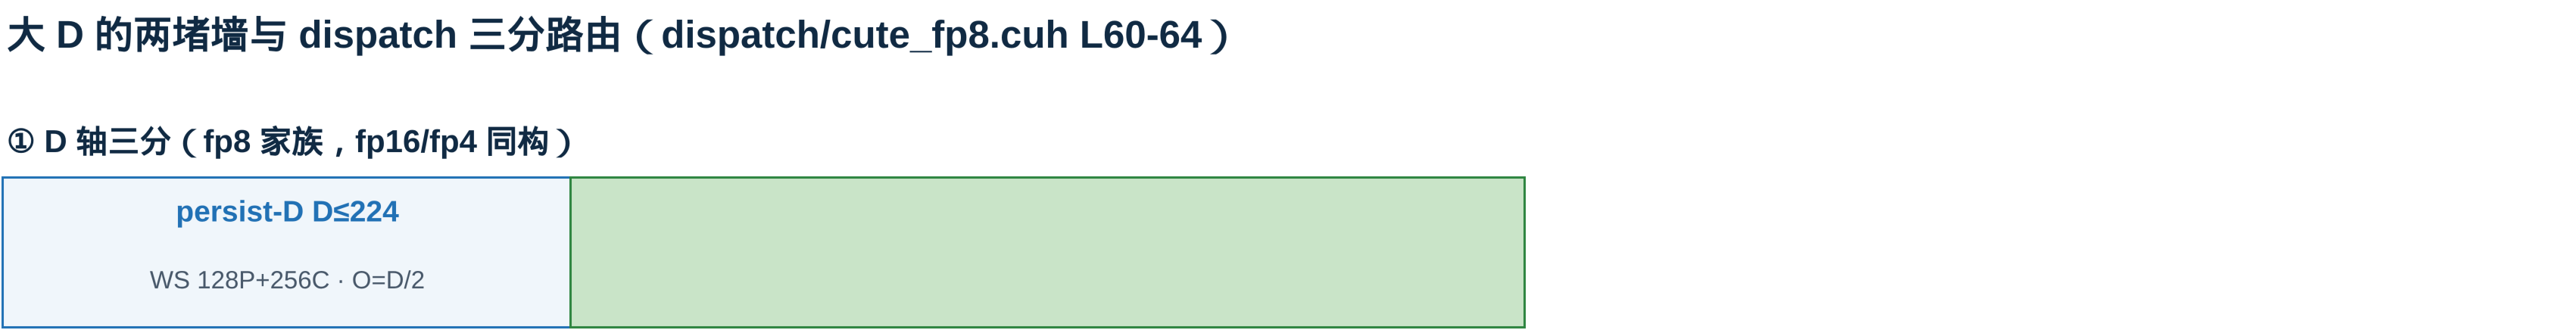
\includegraphics[width=0.98\textwidth]{figures/drawio/fig-30-1-split-d-walls/fig-30-1-split-d-walls.png}
  \begin{tikzpicture}
    \node[anchor=west, inner sep=0pt, align=left, font={\fontsize{7.4}{9.3}\selectfont \bfseries }] at (0.37,-0.354) {大 D 的两堵墙与 dispatch 三分路由（dispatch/cute\_fp8.cuh L60-64）};% w=17.433
    \node[anchor=west, inner sep=0pt, align=left, font={\fontsize{6.1}{7.7}\selectfont \bfseries }] at (0.37,-1.078) {(1) D 轴三分（fp8 家族，fp16/fp4 同构）};% w=4.620
    \node[draw=tkBlue, fill=tkFillBlue, line width=0.5pt, minimum width=3.85cm, minimum height=1.02cm, inner sep=1pt, align=center, text width=3.79cm, font={\fontsize{5.7}{7.1}\selectfont }] at (2.295,-1.833) {};
    \node[anchor=center, inner sep=0pt, align=center, font={\fontsize{5.7}{7.1}\selectfont \bfseries \color{tkBlue} }] at (2.295,-1.555) {persist-D  D$\leq$224};% w=3.665
    \node[anchor=center, inner sep=0pt, align=center, font={\fontsize{4.8}{6.0}\selectfont \color{black!65} }] at (2.295,-2.017) {WS 128P+256C $\cdot$ O=D/2};% w=3.665
    \node[draw=tkGreen, fill=tkFillGreen, line width=0.5pt, minimum width=6.47cm, minimum height=1.02cm, inner sep=1pt, align=center, text width=6.41cm, font={\fontsize{5.7}{7.1}\selectfont }] at (7.454,-1.833) {};
    \node[anchor=center, inner sep=0pt, align=center, font={\fontsize{5.7}{7.1}\selectfont \bfseries \color{tkGreen!70!black} }] at (7.454,-1.555) {split-D M8N1  224$<$D$<$768};% w=6.283
    \node[anchor=center, inner sep=0pt, align=center, font={\fontsize{4.8}{6.0}\selectfont \color{black!65} }] at (7.454,-2.017) {kBr/kBc=128/128 $\cdot$ non-WS 256T $\cdot$ O=D/2};% w=6.283
    \node[draw=tkOrange, fill=tkFillOrange, line width=0.5pt, minimum width=7.39cm, minimum height=1.02cm, inner sep=1pt, align=center, text width=7.33cm, font={\fontsize{5.7}{7.1}\selectfont }] at (13.614,-1.833) {};
    \node[anchor=center, inner sep=0pt, align=center, font={\fontsize{5.7}{7.1}\selectfont \bfseries \color{tkOrange} }] at (13.614,-1.555) {split-D M4N2  D$\geq$768};% w=7.207
    \node[anchor=center, inner sep=0pt, align=center, font={\fontsize{4.8}{6.0}\selectfont \color{black!65} }] at (13.614,-2.017) {kBr/kBc=64/64 $\cdot$ non-WS 256T $\cdot$ O=D/4};% w=7.207
    \node[anchor=center, inner sep=0pt, align=center, font={\fontsize{5.2}{6.6}\selectfont \bfseries }] at (11.15,-1.001) {交叉点 D=768};% w=2.464
    \node[draw=tkRed, fill=tkFillRed, line width=0.5pt, minimum width=8.32cm, minimum height=2.62cm, inner sep=1pt, align=center, text width=8.25cm, font={\fontsize{5.7}{7.1}\selectfont }] at (4.528,-4.235) {};
    \node[anchor=west, inner sep=0pt, align=left, font={\fontsize{6.1}{7.7}\selectfont \bfseries \color{tkRed} }] at (0.616,-3.219) {墙一 smem：K tile 字节 = Bc$\times$D$\times$1B，O(D)};% w=7.823
    \node[anchor=west, inner sep=0pt, align=left, font={\fontsize{5.2}{6.6}\selectfont }] at (0.616,-3.634) {D=512、Bc=128 $\to$ K tile 64KB；加 V stage + Q 即超 99KB 预算};% w=7.823
    \node[anchor=west, inner sep=0pt, align=left, font={\fontsize{5.2}{6.6}\selectfont }] at (0.616,-4.004) {persist-D 的 K stage-0 复用只在 D$\leq$224 挤得过};% w=7.823
    \node[draw=tkRed, fill=none, line width=0.5pt, minimum width=3.70cm, minimum height=0.95cm, inner sep=1pt, align=center, text width=3.63cm, font={\fontsize{5.2}{6.6}\selectfont }] at (2.464,-4.759) {整块 K tile 一次进 smem\\（persist-D：D$\leq$224 专属）};
    \node[draw=tkGreen, fill=none, line width=0.5pt, minimum width=3.70cm, minimum height=0.95cm, inner sep=1pt, align=center, text width=3.63cm, font={\fontsize{5.2}{6.6}\selectfont \bfseries \color{tkGreen!70!black} }] at (6.468,-4.759) {split-D：D 切 chunk 流水\\每 stage 与总 D 无关};
    \node[anchor=west, inner sep=0pt, align=left, font={\fontsize{4.8}{6.0}\selectfont \color{black!55} }] at (0.616,-5.405) {chunk\_index = kv\_tile$\cdot$kDChunks + c，stage/phase 环形推进};% w=7.823
    \node[draw=tkPurple, fill=tkFillPurple, line width=0.5pt, minimum width=8.62cm, minimum height=2.62cm, inner sep=1pt, align=center, text width=8.56cm, font={\fontsize{5.7}{7.1}\selectfont }] at (13.49,-4.235) {};
    \node[anchor=west, inner sep=0pt, align=left, font={\fontsize{6.1}{7.7}\selectfont \bfseries \color{tkPurple} }] at (9.425,-3.219) {墙二 寄存器：O 累加器 = D/(2N\_w) f32/线程};% w=8.131
    \node[anchor=west, inner sep=0pt, align=left, font={\fontsize{5.2}{6.6}\selectfont }] at (9.425,-3.634) {M8N1 单 warp 独占整 D 列：D=512 $\to$ 256 regs 压线（上限 255）};% w=8.131
    \node[anchor=west, inner sep=0pt, align=left, font={\fontsize{5.2}{6.6}\selectfont }] at (9.425,-4.004) {D$\geq$896 大量 spill 崩塌（D=1024 实测 \textasciitilde{}100T）};% w=8.131
    \node[draw=tkPurple, fill=none, line width=0.5pt, minimum width=3.85cm, minimum height=0.95cm, inner sep=1pt, align=center, text width=3.79cm, font={\fontsize{5.2}{6.6}\selectfont }] at (11.35,-4.759) {M8N1 (8,1,1)：O=D/2\\D=1024 $\to$ 512 regs 溢出};
    \node[draw=tkOrange, fill=none, line width=0.5pt, minimum width=3.85cm, minimum height=0.95cm, inner sep=1pt, align=center, text width=3.79cm, font={\fontsize{5.2}{6.6}\selectfont \bfseries \color{tkOrange!75!black} }] at (15.508,-4.759) {M4N2 (4,2,1)：O=D/4\\D=1024 $\to$ 256 regs 边缘 spill 154T};
    \node[draw=gray!55, fill=black!2, line width=0.5pt, minimum width=17.43cm, minimum height=2.31cm, inner sep=1pt, align=center, text width=17.37cm, font={\fontsize{5.7}{7.1}\selectfont }] at (9.086,-7.253) {};
    \node[anchor=west, inner sep=0pt, align=left, font={\fontsize{6.1}{7.7}\selectfont \bfseries }] at (0.616,-6.391) {(2) 寄存器压力模型：N\_w 消去，只有减 M\_w 有效};% w=16.940
    \node[anchor=west, inner sep=0pt, align=left, font={\fontsize{5.7}{7.1}\selectfont }] at (0.616,-6.868) {per-thread：O\_acc = 4$\cdot$(kBr/16M\_w)$\cdot$(D/8N\_w)/(kBr/16M\_w) = D/(2N\_w)};% w=9.856
    \node[anchor=west, inner sep=0pt, align=left, font={\fontsize{5.7}{7.1}\selectfont \bfseries \color{tkPurple} }] at (0.616,-7.269) {per-SM 池占比：[D/(2N\_w)] / [65536/(32M\_wN\_w)] = D$\cdot$M\_w/4096};% w=9.856
    \node[anchor=west, inner sep=0pt, align=left, font={\fontsize{5.2}{6.6}\selectfont \color{black!65} }] at (0.616,-7.669) {N\_w 精确消去：M4N4 $\equiv$ M4N2（同为 D/1024）；M2N4 $\to$ D/2048 是 D$>$1024 正解};% w=9.856
    \node[anchor=west, inner sep=0pt, align=left, font={\fontsize{5.2}{6.6}\selectfont \bfseries \color{tkRed} }] at (10.965,-7.099) {被否决的捷径(1)：QK M8N1 + PV M4N2 混合布局};% w=6.591
    \node[anchor=west, inner sep=0pt, align=left, font={\fontsize{4.8}{6.0}\selectfont }] at (10.965,-7.623) {QK/PV 共享 Q tile，M 维须一致：\\kBr=128 $\to$ PV 仍 D/2\\kBr=64 $\to$ M8N1 空 4 warp};% w=6.591
    \node[anchor=west, inner sep=0pt, align=left, font={\fontsize{5.2}{6.6}\selectfont \bfseries \color{tkRed} }] at (10.965,-8.177) {被否决的捷径(2)：WS 版 split-D};% w=6.591
    \node[anchor=west, inner sep=0pt, align=left, font={\fontsize{4.8}{6.0}\selectfont }] at (10.965,-8.747) {setmaxnreg 上限 232 装不下 D=512 的 256-reg O};% w=6.591
    \node[draw=tkGreen, fill=tkFillGreen, line width=0.5pt, minimum width=17.43cm, minimum height=2.31cm, inner sep=1pt, align=center, text width=17.37cm, font={\fontsize{5.7}{7.1}\selectfont }] at (9.086,-10.025) {};
    \node[anchor=west, inner sep=0pt, align=left, font={\fontsize{6.1}{7.7}\selectfont \bfseries \color{tkGreen!70!black} }] at (0.616,-9.163) {(3) 实测交叉点（5090，fp16 同构；PRO 5000 数据见正文 30.6）};% w=16.940
    \node[anchor=west, inner sep=0pt, align=left, font={\fontsize{5.2}{6.6}\selectfont }] at (0.616,-9.579) {D$\leq$640：M8N1 快 +2\textasciitilde{}16\%（无 P roundtrip、kBr 大一倍）};% w=8.316
    \node[anchor=west, inner sep=0pt, align=left, font={\fontsize{5.2}{6.6}\selectfont \bfseries }] at (0.616,-9.948) {D$\geq$768：M4N2 快 +7\%@768、+11\%@896、+55\%@1024};% w=8.316
    \node[anchor=west, inner sep=0pt, align=left, font={\fontsize{5.2}{6.6}\selectfont \color{black!55} }] at (0.616,-10.318) {FFPA\_FP8\_FORCE\_KERNEL=split\_d|m4n2（224$<$D$\leq$1024）可强制 A/B};% w=8.316
    \node[anchor=west, inner sep=0pt, align=left, font={\fontsize{5.2}{6.6}\selectfont \color{black!55} }] at (0.616,-10.688) {PRO 5000 实测（本机 headdim 止于 512）：D=512 self 203T / 2.98x};% w=8.316
    \node[anchor=west, inner sep=0pt, align=left, font={\fontsize{5.7}{7.1}\selectfont \bfseries \color{tkGreen!70!black} }] at (9.548,-9.579) {split-D 是精确变换：};% w=8.008
    \node[anchor=west, inner sep=0pt, align=left, font={\fontsize{5.2}{6.6}\selectfont }] at (9.548,-9.948) {QK 侧 D 是归约维：$\Sigma$\_c Q\_c K\_c\^{}T 累加进同一 S（无新舍入点）};% w=8.008
    \node[anchor=west, inner sep=0pt, align=left, font={\fontsize{5.2}{6.6}\selectfont }] at (9.548,-10.318) {PV 侧 D 是输出列维：各 chunk 的 O 段独立累加};% w=8.008
    \node[anchor=west, inner sep=0pt, align=left, font={\fontsize{5.2}{6.6}\selectfont \bfseries }] at (9.548,-10.688) {softmax 行统计 (m,$\ell$) 是 KV 行维的量------与 D 切分无关};% w=8.008
    \draw[black!75, line width=0.8pt, dashed] (9.918,-1.14) -- (9.918,-2.464);
    \draw[gray!55, line width=0.5pt, dashed] (4.22,-1.14) -- (4.22,-2.464);
    \draw[tkGreen, line width=0.8pt, -{Stealth[length=2.2pt,width=1.8pt]}] (4.312,-4.759) -- (4.62,-4.759);
    \draw[tkOrange, line width=0.8pt, -{Stealth[length=2.2pt,width=1.8pt]}] (13.275,-4.759) -- (13.583,-4.759);
    \draw[gray!55, line width=0.5pt] (10.718,-6.714) -- (10.718,-8.1);
    \draw[gray!55, line width=0.5pt] (9.302,-9.425) -- (9.302,-10.842);
  \end{tikzpicture}
  \caption{大 $D$ 的两堵墙与 dispatch 三分路由。smem 墙由 split-D 拆
  （chunk 流水，smem 与 $D$ 解耦）；寄存器墙由 M4N2 拆（$N_w=2$ 把
  per-thread $O$ 从 $D/2$ 减到 $D/4$）；$D=768$ 是实测交叉点。}
  \label{fig:30-walls}
\end{figure}

\begin{figure}[htbp]
  \centering
  % was: 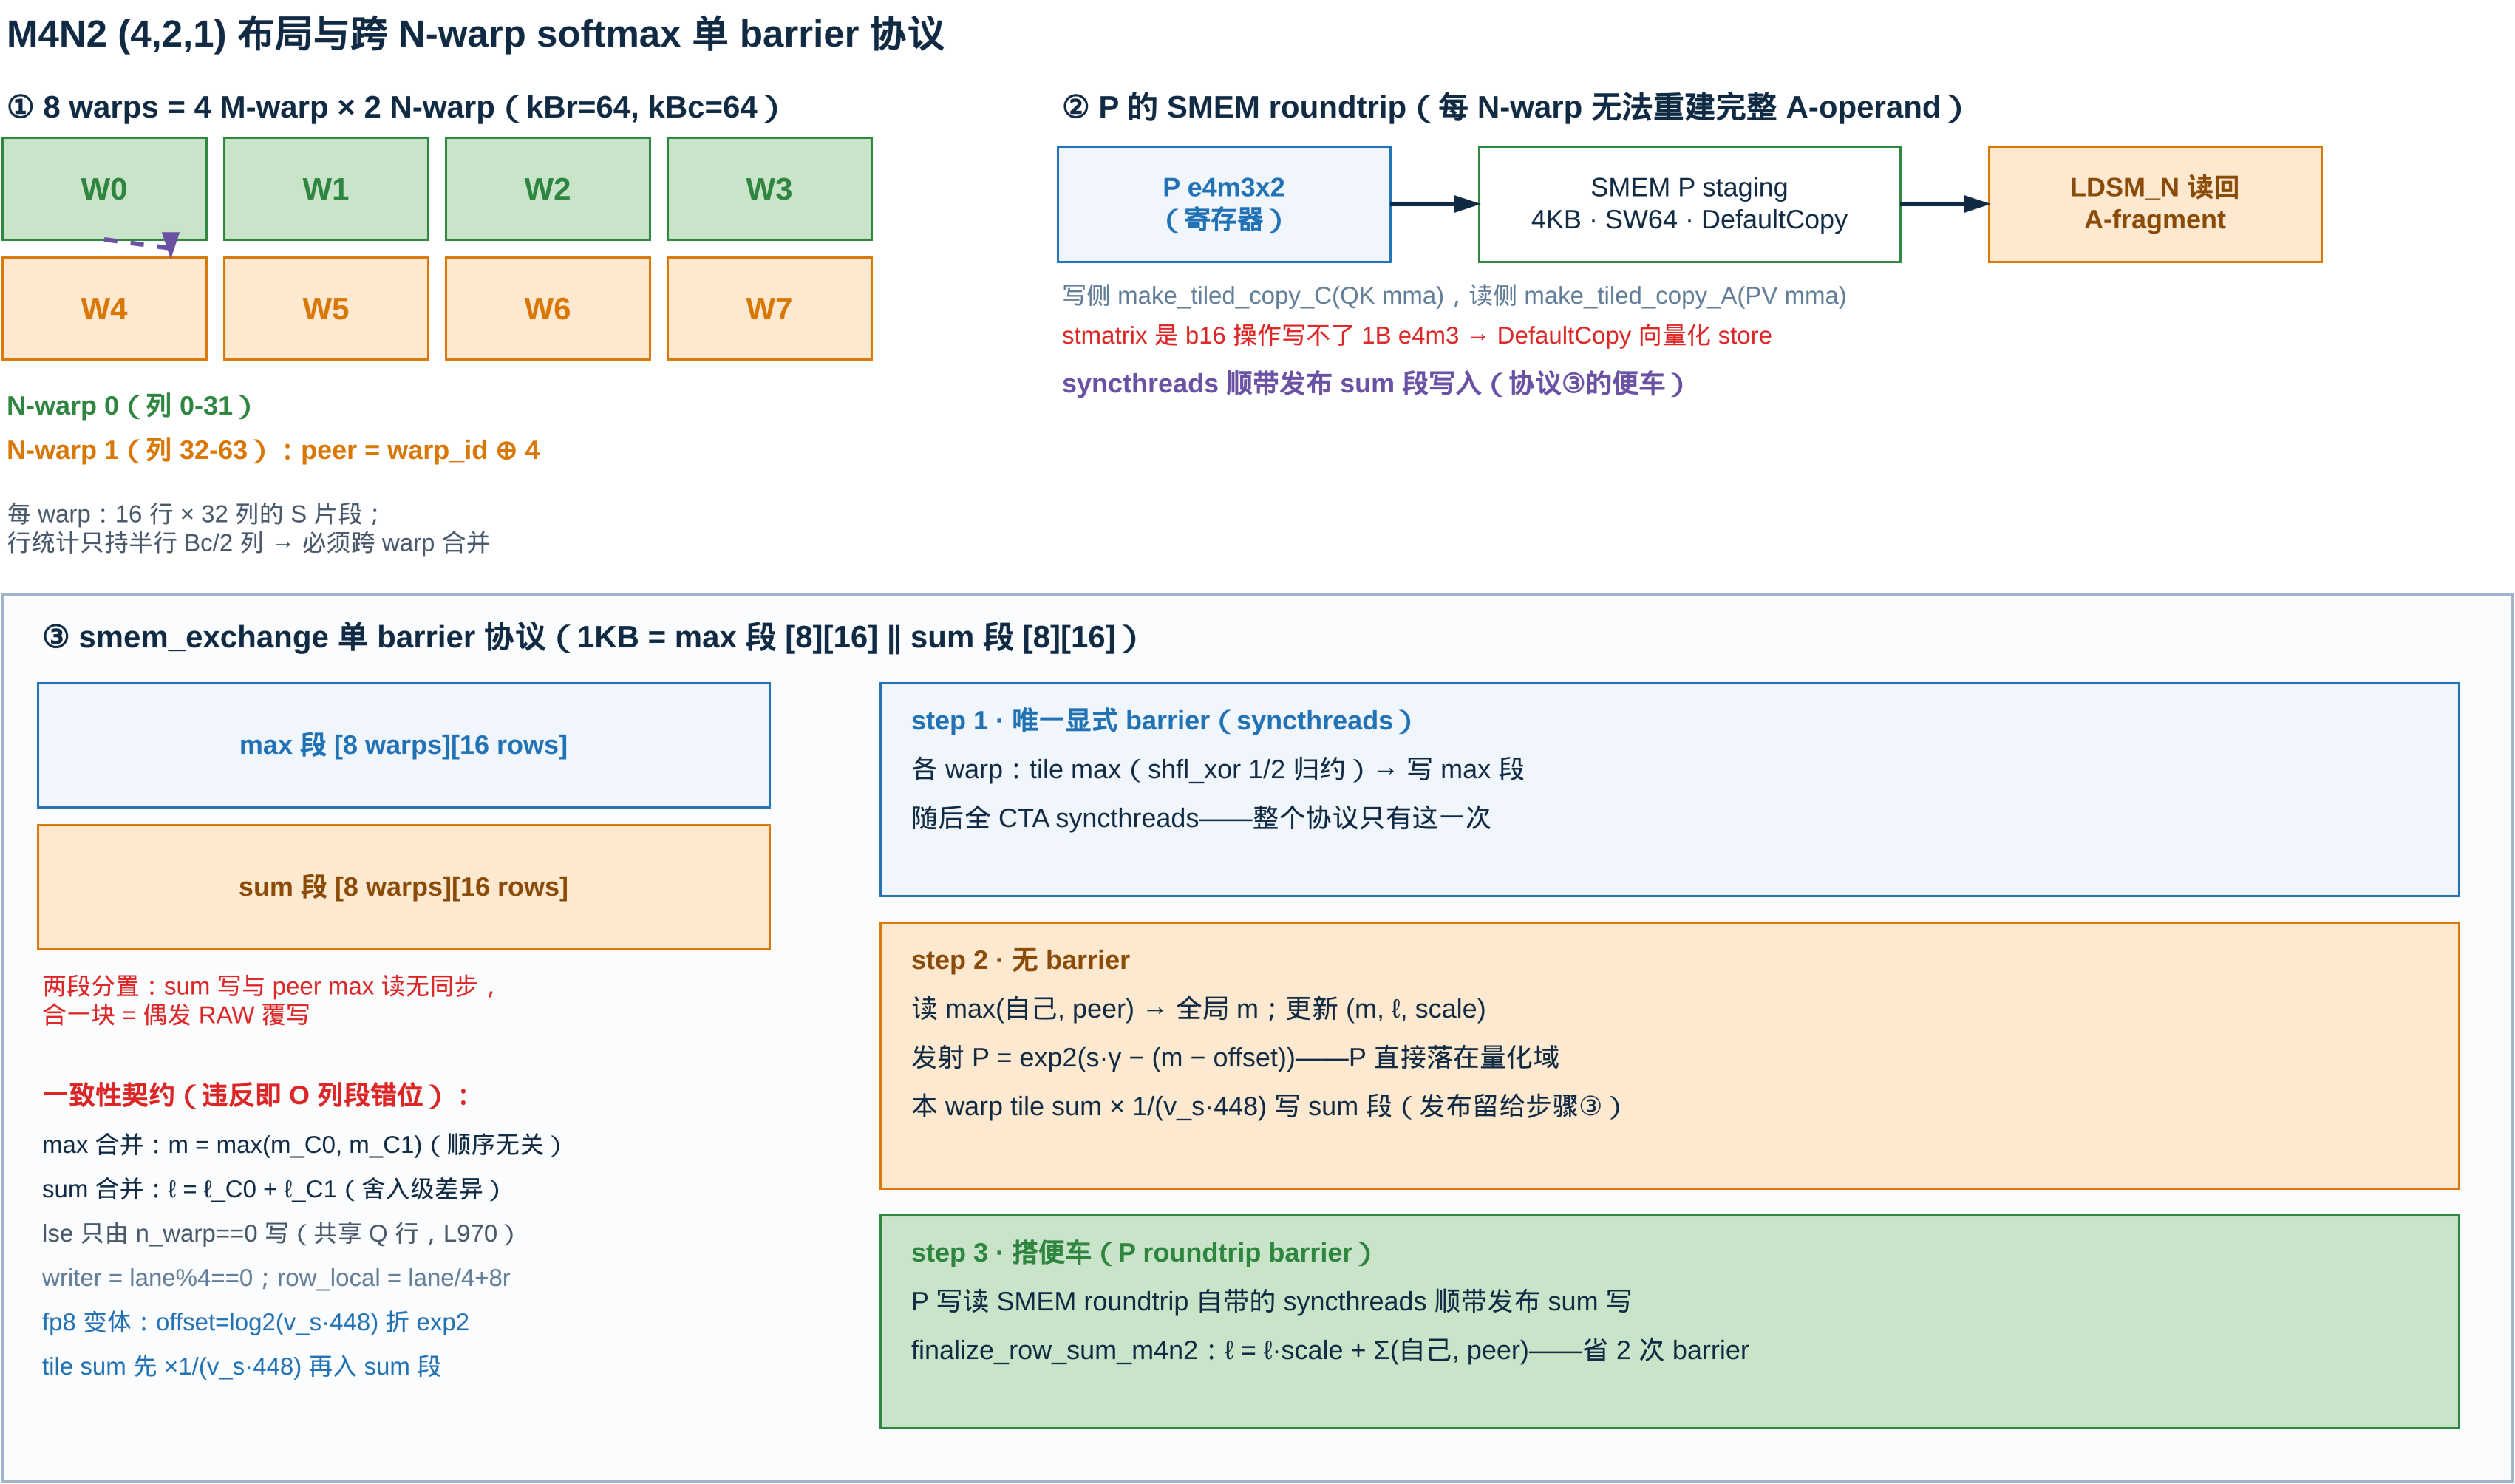
\includegraphics[width=0.98\textwidth]{figures/drawio/fig-30-2-m4n2-softmax/fig-30-2-m4n2-softmax.png}
  \begin{tikzpicture}
    \node[anchor=west, inner sep=0pt, align=left, font={\fontsize{7.4}{9.3}\selectfont \bfseries }] at (0.37,-0.354) {M4N2 (4,2,1) 布局与跨 N-warp softmax 单 barrier 协议};% w=17.433
    \node[anchor=west, inner sep=0pt, align=left, font={\fontsize{5.6}{7.0}\selectfont \bfseries }] at (0.37,-0.862) {(1) 8 warps = 4 M-warp $\times$ 2 N-warp（kBr=64, kBc=64）};% w=8.624
    \node[draw=tkGreen, fill=tkFillGreen, line width=0.5pt, minimum width=1.42cm, minimum height=0.71cm, inner sep=1pt, align=center, text width=1.36cm, font={\fontsize{6.1}{7.7}\selectfont \bfseries \color{tkGreen!70!black} }] at (1.078,-1.432) {W0};
    \node[draw=tkGreen, fill=tkFillGreen, line width=0.5pt, minimum width=1.42cm, minimum height=0.71cm, inner sep=1pt, align=center, text width=1.36cm, font={\fontsize{6.1}{7.7}\selectfont \bfseries \color{tkGreen!70!black} }] at (2.618,-1.432) {W1};
    \node[draw=tkGreen, fill=tkFillGreen, line width=0.5pt, minimum width=1.42cm, minimum height=0.71cm, inner sep=1pt, align=center, text width=1.36cm, font={\fontsize{6.1}{7.7}\selectfont \bfseries \color{tkGreen!70!black} }] at (4.158,-1.432) {W2};
    \node[draw=tkGreen, fill=tkFillGreen, line width=0.5pt, minimum width=1.42cm, minimum height=0.71cm, inner sep=1pt, align=center, text width=1.36cm, font={\fontsize{6.1}{7.7}\selectfont \bfseries \color{tkGreen!70!black} }] at (5.698,-1.432) {W3};
    \node[draw=tkOrange, fill=tkFillOrange, line width=0.5pt, minimum width=1.42cm, minimum height=0.71cm, inner sep=1pt, align=center, text width=1.36cm, font={\fontsize{6.1}{7.7}\selectfont \bfseries \color{tkOrange} }] at (1.078,-2.264) {W4};
    \node[draw=tkOrange, fill=tkFillOrange, line width=0.5pt, minimum width=1.42cm, minimum height=0.71cm, inner sep=1pt, align=center, text width=1.36cm, font={\fontsize{6.1}{7.7}\selectfont \bfseries \color{tkOrange} }] at (2.618,-2.264) {W5};
    \node[draw=tkOrange, fill=tkFillOrange, line width=0.5pt, minimum width=1.42cm, minimum height=0.71cm, inner sep=1pt, align=center, text width=1.36cm, font={\fontsize{6.1}{7.7}\selectfont \bfseries \color{tkOrange} }] at (4.158,-2.264) {W6};
    \node[draw=tkOrange, fill=tkFillOrange, line width=0.5pt, minimum width=1.42cm, minimum height=0.71cm, inner sep=1pt, align=center, text width=1.36cm, font={\fontsize{6.1}{7.7}\selectfont \bfseries \color{tkOrange} }] at (5.698,-2.264) {W7};
    \node[anchor=west, inner sep=0pt, align=left, font={\fontsize{5.2}{6.6}\selectfont \bfseries \color{tkGreen!70!black} }] at (0.37,-2.941) {N-warp 0（列 0-31）};% w=6.406
    \node[anchor=west, inner sep=0pt, align=left, font={\fontsize{5.2}{6.6}\selectfont \bfseries \color{tkOrange} }] at (0.37,-3.249) {N-warp 1（列 32-63）：peer = warp\_id $\oplus$ 4};% w=6.406
    \node[anchor=west, inner sep=0pt, align=left, font={\fontsize{4.8}{6.0}\selectfont \color{black!65} }] at (0.37,-3.788) {每 warp：16 行 $\times$ 32 列的 S 片段；\\行统计只持半行 Bc/2 列 $\to$ 必须跨 warp 合并};% w=6.622
    \node[anchor=west, inner sep=0pt, align=left, font={\fontsize{6.1}{7.7}\selectfont \bfseries }] at (7.7,-0.862) {(2) P 的 SMEM roundtrip（每 N-warp 无法重建完整 A-operand）};% w=10.102
    \node[draw=tkBlue, fill=tkFillBlue, line width=0.5pt, minimum width=2.31cm, minimum height=0.80cm, inner sep=1pt, align=center, text width=2.25cm, font={\fontsize{5.2}{6.6}\selectfont \bfseries \color{tkBlue} }] at (8.855,-1.54) {P e4m3x2\\（寄存器）};
    \node[draw=tkGreen, fill=none, line width=0.5pt, minimum width=2.93cm, minimum height=0.80cm, inner sep=1pt, align=center, text width=2.86cm, font={\fontsize{5.0}{6.3}\selectfont }] at (12.089,-1.54) {SMEM P staging\\4KB $\cdot$ SW64 $\cdot$ DefaultCopy};
    \node[draw=tkOrange, fill=tkFillOrange, line width=0.5pt, minimum width=2.31cm, minimum height=0.80cm, inner sep=1pt, align=center, text width=2.25cm, font={\fontsize{5.2}{6.6}\selectfont \bfseries \color{tkOrange!75!black} }] at (15.323,-1.54) {LDSM\_N 读回\\A-fragment};
    \node[anchor=west, inner sep=0pt, align=left, font={\fontsize{4.8}{6.0}\selectfont \color{black!55} }] at (7.7,-2.171) {写侧 make\_tiled\_copy\_C(QK mma)，读侧 make\_tiled\_copy\_A(PV mma)};% w=8.778
    \node[anchor=west, inner sep=0pt, align=left, font={\fontsize{4.8}{6.0}\selectfont \color{tkRed} }] at (7.7,-2.449) {stmatrix 是 b16 操作写不了 1B e4m3 $\to$ DefaultCopy 向量化 store};% w=8.778
    \node[anchor=west, inner sep=0pt, align=left, font={\fontsize{5.2}{6.6}\selectfont \bfseries \color{tkPurple} }] at (7.7,-2.787) {syncthreads 顺带发布 sum 段写入（协议(3)的便车）};% w=8.778
    \node[draw=gray!55, fill=black!2, line width=0.5pt, minimum width=17.43cm, minimum height=6.16cm, inner sep=1pt, align=center, text width=17.37cm, font={\fontsize{5.7}{7.1}\selectfont }] at (9.086,-7.33) {};
    \node[anchor=west, inner sep=0pt, align=left, font={\fontsize{6.1}{7.7}\selectfont \bfseries }] at (0.616,-4.543) {(3) smem\_exchange 单 barrier 协议（1KB = max 段 [8][16] $\|$ sum 段 [8][16]）};% w=16.940
    \node[draw=tkBlue, fill=tkFillBlue, line width=0.5pt, minimum width=5.08cm, minimum height=0.86cm, inner sep=1pt, align=center, text width=5.02cm, font={\fontsize{5.2}{6.6}\selectfont \bfseries \color{tkBlue} }] at (3.157,-5.298) {max 段 [8 warps][16 rows]};
    \node[draw=tkOrange, fill=tkFillOrange, line width=0.5pt, minimum width=5.08cm, minimum height=0.86cm, inner sep=1pt, align=center, text width=5.02cm, font={\fontsize{5.2}{6.6}\selectfont \bfseries \color{tkOrange!75!black} }] at (3.157,-6.283) {sum 段 [8 warps][16 rows]};
    \node[anchor=west, inner sep=0pt, align=left, font={\fontsize{4.8}{6.0}\selectfont \color{tkRed} }] at (0.616,-7.069) {两段分置：sum 写与 peer max 读无同步，\\合一块 = 偶发 RAW 覆写};% w=5.174
    \node[anchor=west, inner sep=0pt, align=left, font={\fontsize{5.2}{6.6}\selectfont \bfseries \color{tkRed} }] at (0.616,-7.731) {一致性契约（违反即 O 列段错位）：};% w=5.236
    \node[anchor=west, inner sep=0pt, align=left, font={\fontsize{4.8}{6.0}\selectfont }] at (0.616,-8.07) {max 合并：m = max(m\_C0, m\_C1)（顺序无关）};% w=5.236
    \node[anchor=west, inner sep=0pt, align=left, font={\fontsize{4.8}{6.0}\selectfont }] at (0.616,-8.378) {sum 合并：$\ell$ = $\ell$\_C0 + $\ell$\_C1（舍入级差异）};% w=5.236
    \node[anchor=west, inner sep=0pt, align=left, font={\fontsize{4.8}{6.0}\selectfont \color{black!65} }] at (0.616,-8.686) {lse 只由 n\_warp==0 写（共享 Q 行，L970）};% w=5.236
    \node[anchor=west, inner sep=0pt, align=left, font={\fontsize{4.8}{6.0}\selectfont \color{black!55} }] at (0.616,-8.994) {writer = lane\%4==0；row\_local = lane/4+8r};% w=5.236
    \node[anchor=west, inner sep=0pt, align=left, font={\fontsize{4.8}{6.0}\selectfont \color{tkBlue} }] at (0.616,-9.302) {fp8 变体：offset=log2(v\_s$\cdot$448) 折 exp2};% w=5.236
    \node[anchor=west, inner sep=0pt, align=left, font={\fontsize{4.8}{6.0}\selectfont \color{tkBlue} }] at (0.616,-9.61) {tile sum 先 $\times$1/(v\_s$\cdot$448) 再入 sum 段};% w=5.236
    \node[draw=tkBlue, fill=tkFillBlue, line width=0.5pt, minimum width=10.96cm, minimum height=1.48cm, inner sep=1pt, align=center, text width=10.90cm, font={\fontsize{5.7}{7.1}\selectfont }] at (11.95,-5.606) {};
    \node[anchor=west, inner sep=0pt, align=left, font={\fontsize{5.2}{6.6}\selectfont \bfseries \color{tkBlue} }] at (6.653,-5.128) {step 1 $\cdot$ 唯一显式 barrier（syncthreads）};% w=10.595
    \node[anchor=west, inner sep=0pt, align=left, font={\fontsize{5.2}{6.6}\selectfont }] at (6.653,-5.467) {各 warp：tile max（shfl\_xor 1/2 归约）$\to$ 写 max 段};% w=10.595
    \node[anchor=west, inner sep=0pt, align=left, font={\fontsize{5.2}{6.6}\selectfont }] at (6.653,-5.806) {随后全 CTA syncthreads------整个协议只有这一次};% w=10.595
    \node[draw=tkOrange, fill=tkFillOrange, line width=0.5pt, minimum width=10.96cm, minimum height=1.85cm, inner sep=1pt, align=center, text width=10.90cm, font={\fontsize{5.7}{7.1}\selectfont }] at (11.95,-7.454) {};
    \node[anchor=west, inner sep=0pt, align=left, font={\fontsize{5.2}{6.6}\selectfont \bfseries \color{tkOrange!75!black} }] at (6.653,-6.791) {step 2 $\cdot$ 无 barrier};% w=10.595
    \node[anchor=west, inner sep=0pt, align=left, font={\fontsize{5.2}{6.6}\selectfont }] at (6.653,-7.13) {读 max(自己, peer) $\to$ 全局 m；更新 (m, $\ell$, scale)};% w=10.595
    \node[anchor=west, inner sep=0pt, align=left, font={\fontsize{5.2}{6.6}\selectfont }] at (6.653,-7.469) {发射 P = exp2(s$\cdot$$\gamma$ $-$ (m $-$ offset))------P 直接落在量化域};% w=10.595
    \node[anchor=west, inner sep=0pt, align=left, font={\fontsize{5.2}{6.6}\selectfont }] at (6.653,-7.808) {本 warp tile sum $\times$ 1/(v\_s$\cdot$448) 写 sum 段（发布留给步骤(3)）};% w=10.595
    \node[draw=tkGreen, fill=tkFillGreen, line width=0.5pt, minimum width=10.96cm, minimum height=1.48cm, inner sep=1pt, align=center, text width=10.90cm, font={\fontsize{5.7}{7.1}\selectfont }] at (11.95,-9.302) {};
    \node[anchor=west, inner sep=0pt, align=left, font={\fontsize{5.2}{6.6}\selectfont \bfseries \color{tkGreen!70!black} }] at (6.653,-8.824) {step 3 $\cdot$ 搭便车（P roundtrip barrier）};% w=10.595
    \node[anchor=west, inner sep=0pt, align=left, font={\fontsize{5.2}{6.6}\selectfont }] at (6.653,-9.163) {P 写读 SMEM roundtrip 自带的 syncthreads 顺带发布 sum 写};% w=10.595
    \node[anchor=west, inner sep=0pt, align=left, font={\fontsize{5.2}{6.6}\selectfont }] at (6.653,-9.502) {finalize\_row\_sum\_m4n2：$\ell$ = $\ell$$\cdot$scale + $\Sigma$(自己, peer)------省 2 次 barrier};% w=10.595
    \draw[tkPurple, line width=0.8pt, dashed, -{Stealth[length=2.2pt,width=1.8pt]}] (1.078,-1.786) -- (1.54,-1.848) -- (1.54,-1.91);
    \draw[black!75, line width=0.8pt, -{Stealth[length=2.2pt,width=1.8pt]}] (10.01,-1.54) -- (10.626,-1.54);
    \draw[black!75, line width=0.8pt, -{Stealth[length=2.2pt,width=1.8pt]}] (13.552,-1.54) -- (14.168,-1.54);
  \end{tikzpicture}
  \caption{M4N2 的 $(4,2,1)$ atom 布局与跨 N-warp softmax 单 barrier
  协议。max 段与 sum 段分置 \texttt{smem\_exchange} 防 RAW；sum 的
  发布搭 P roundtrip barrier 的便车。}
  \label{fig:30-m4n2}
\end{figure}

\FloatBarrier

\section{性能分析}

\subsection{本机实测（RTX PRO 5000，B1 H32 N8192，bench 默认配置）}

命令：
\begin{lstlisting}[style=console,aboveskip=4pt,belowskip=2pt]
export CUDA_VISIBLE_DEVICES=7 FFPA_CUDA_ALLOW_SMALL_D=1
python -m ffpa_attn.bench --fwd-backend cuda --cuda-impl fp8 \
  --tasks self-attn,causal --D {256,320,512} --no-bwd --show-allclose
\end{lstlisting}

\begin{center}
\begin{tabular}{@{}llrrrl@{}}
\toprule
$D$ & task & FFPA ms & SDPA ms & TFLOPS & speedup \\
\midrule
256 & self   & 8.12  & 10.52 & 271T & 1.30x \\
256 & causal & 4.73  & 5.29  & 233T & 1.12x \\
320 & self   & 10.71 & 40.25 & 257T & 3.76x \\
320 & causal & 6.23  & 20.61 & 221T & 3.31x \\
512 & self   & 21.71 & 64.74 & 203T & 2.98x \\
512 & causal & 12.82 & 32.92 & 172T & 2.57x \\
\bottomrule
\end{tabular}
\end{center}

三条读数：其一，self-attn 的 speedup 从 $D=256$ 的 1.30x 跳到
$D=320$ 的 3.76x——拐点不在 kernel 而在\textbf{参照系}：SDPA 在
$D\notin\{64,128\}$ 时掉出最优 kernel 选择，fp8 的 1B 元素带宽优势
立即显形。其二，TFLOPS 随 $D$ 单调下降（271$\to$203T）：$D$ 越大
softmax 与 P 量化等 $O(B_c)$ 项占比越高、$O$ 寄存器压力越大，这是
split-D 无法消除的税。其三，causal 的 allclose 在 D=320 bf16 与
D=512 fp16 两格临界失败——见 30.2.3~节的已知边界说明；dense 六格
全绿，数据落盘 \texttt{.tmp/book-bench/ch30/}。

\subsection{交叉点与 M4N2 的引用数据（本机无 $D\ge768$ 编译实例）}

本机 headdim 编译集止于 512，M4N2 只能引用 5090 数据（fp16 家族同构、
同一 dispatch 交叉点）：$D\le640$ 时 M8N1 快 $2\sim16\%$；
$D\ge768$ 时 M4N2 快 $+7\%@768$、$+11\%@896$、$+55\%@1024$。崩塌侧
的数字更有教学价值：$D=1024$ 时 M8N1 的 $O_{\text{acc}}=512$ regs
溢出 local memory，吞吐 $\sim$100T；M4N2 同 $D$ 边缘 spill 仍有
154T。\texttt{FFPA\_FP8\_FORCE\_KERNEL=split\_d|m4n2}（$224<D\le1024$，
\texttt{dispatch/cute\_fp8.cuh} L24--33，仅在 \texttt{--debug-ext fp8}
的 debug 构建里生效）可在有 768+ 编译实例的
机器上强制 A/B 复现交叉点。

\subsection{roofline 视角}

fp8 split-D 在 $D=512$ 的 203T 大约是 fp8 persist-D 峰值（365T，
表~29.2）的 56\%。差价的构成：$O$ 累加器随 $D$ 翻倍的寄存器税
（occupancy 1 CTA）、chunk 循环多出的 barrier 握手、以及 epilogue
批量 staging 的 smem 往返。这不是 split-D 的失败——绝对吞吐仍高于
fp16 家族同 $D$ 量级，带宽侧（1B/元素）更是 3.76x speedup 的直接
来源。

\section{实践经验}

\subsection{案例：causal allclose 临界失败的定位与定性}

30.6~节表格里有两格 \texttt{allclose} 失败：D=320（bf16）、
D=512（fp16）。

定性过程值得记录，脚本在 \texttt{.tmp/book-bench/ch30/}：

\begin{enumerate}[itemsep=0pt,topsep=2pt]
  \item \textbf{先看模式不看标量}。对 $D\in\{256,320,512\}$ 各跑
        causal，逐 512-行块统计超阈行占比：三者模式\textbf{完全一致}
        ——前 $\sim$30\% 块 100\% 超阈、后段 0\%，max $\sim$2、
        mean $\sim$0.007；
  \item \textbf{dense 对照}。self-attn 六格全绿 $\Rightarrow$ 排除
        kernel 结构性错误（chunk 流水、mask、epilogue 都对）；
  \item \textbf{对照头注释}。L40--43 声明的「causal 早期行
        attend 少、误差不被平均」与实测模式吻合：早期行
        $P$ 分布尖，e4m3 的 $2^{-3}$ 相对舍入直接进 $O$；行号
        过半后 $P$ 足够平，误差被平均掉；
  \item \textbf{结论}：已知精度特性，非回归 bug。需要严格
        causal 精度的场景走 hybrid（前若干行 fp16 stage-1）。
\end{enumerate}

这套流程（模式 $\to$ dense 对照 $\to$ 对照声明 $\to$ 定性）与
29.7.1~节 D=192 的五步法同构：先证明「不是 bug」再决定要不要修。

\subsection{什么时候不该学本章}

split-D/M4N2 是 $D>224$ 的\textbf{被迫选择}，不是普适更优。三条负面
证据：WS 版 split-D 被 setmaxnreg 232 上限否决；QK/PV 混合 atom 布局
被 M 维一致性否决；fused-rescale 在 split-D 域被单 CTA 藏不住的
tensor pipe 压力否决。三条都是「在 persist-D 域成立的优化不能平移」
的实例——迁移优化前先核对 occupancy 与寄存器结构是否同型。

\section{常见坑}

\begin{enumerate}[itemsep=2pt,topsep=2pt]
  \item \textbf{P roundtrip 写侧坐标系}：写侧必须从 QK 的
        \texttt{tiled\_mma\_qk} 构造 \texttt{make\_tiled\_copy\_C}，
        读侧从 PV 的 \texttt{tiled\_mma\_pv} 构造
        \texttt{make\_tiled\_copy\_A}；手写 A-operand 映射与 LDSM
        读侧不对称会数值爆炸（sm80 家族血泪，L685--698 用
        \texttt{DefaultCopy} 规避向量化陷阱）。
  \item \textbf{max/sum 同区覆写}：单 barrier 协议里 sum 写与 peer
        max 读之间没有同步，两段必须分置；合成一块省下的 512B 换来
        偶发 RAW 错值（softmax.cuh L92--95）。
  \item \textbf{stmatrix 写不了 1B e4m3}：它是 b16 操作；1B 元素的
        P staging 退回 \texttt{DefaultCopy} 向量化 store（L685--688）。
  \item \textbf{两套块宽不一致}：$k_{Br}=64$ vs 量化 128 行块，奇数
        tile 需要 \texttt{quant\_offset}/\texttt{quant\_rb} 重映射
        （L129、L300--307）；漏掉的行查到邻块的 scale，误差温和到
        很难肉眼发现。
  \item \textbf{kSmemElems 的单位}：fp8 traits 里它数 1B 元素恰等于
        字节数；O staging 断言要乘 \texttt{sizeof(ElementO)}，否则
        预算虚大一倍（L105--108）。
  \item \textbf{stage 下限的家族差异}：persist-D 抬 stages 已证伪、
        m4n2 抬到 3 是全局最优——差别只在 occupancy 是否已被锁死；
        跨家族抄 stage 配置前先想清楚这一条。
\end{enumerate}

\section{面试要点速查}

\begin{enumerate}[itemsep=2pt,topsep=2pt]
  \item \textbf{split-D 为什么精确}？QK 侧 $D$ 是归约维，chunk 累加
        进同一 fragment（式~\ref{eq:30-qk-split}）；PV 侧是输出列维，
        各 chunk 独立（式~\ref{eq:30-pv-split}）；softmax 行统计与
        $D$ 切分无关——不产生 per-chunk 的 $(m,\ell)$。
  \item \textbf{M4N2 减的是哪一维}？$N$ 维（输出列劈 2 warp），
        per-thread $O$ 从 $D/2$ 到 $D/4$；但 per-SM 池占比
        $D\cdot M_w/4096$ 里 $N_w$ 消去（式~\ref{eq:30-smpool}），
        只有减 $M_w$ 才降总量——所以 $D>1024$ 的正解是 M2N4。
  \item \textbf{跨 N-warp softmax 协议}？max 段交换 + 单 barrier；
        sum 搭 P roundtrip barrier 的便车由 \texttt{finalize} 折叠；
        两 N-warp 必须持有相同 $(m,\ell)$ 否则 rescale 因子分裂。
  \item \textbf{P 为什么要过 SMEM}？M4N2 每 N-warp 只持半行
        $B_c$ 列，A-operand 无法 warp 内重建；roundtrip 4KB/tile。
  \item \textbf{交叉点为何在 $D=768$}？之下 M8N1 无 roundtrip 且
        $k_{Br}=128$ 效率高；之上 $D/2$ 逼近/超过 255 寄存器上限，
        M4N2 的 $D/4$ 开始统治（5090：+7\%@768 $\to$ +55\%@1024）。
  \item \textbf{split-D 为何非 WS}？setmaxnreg consumer 上限 232
        装不下 $D\ge512$ 的 256-reg $O$ 累加器；全线程 MMA +
        tid==0 发 TMA 是被迫也是合理。
  \item \textbf{fp8 causal 早期行为何误差大}？attend 的 key 少，
        $P$ 分布尖，e4m3 相对舍入不被平均；dense 无此问题；
        工程解法是 hybrid 前若干行 fp16。
\end{enumerate}

\section{最小测试与动手实验}

\begin{enumerate}[itemsep=2pt,topsep=2pt]
  \item \textbf{bench 复跑}（卡 7）：30.6~节命令逐 $D$ 复现表格；
        观察 self speedup 在 $D=256\to320$ 的跳变并解释参照系切换。
  \item \textbf{误差模式复现}：用 \texttt{CUDABackend(enable\_fp8=True)}
        直接调 \texttt{ffpa\_attn\_func}，对 causal 输出按 512-行块
        统计超阈行占比，画出前 30\% 块 100\% 的直方图
        （\texttt{.tmp/book-bench/ch30/d512\_causal\_check.py}）。
  \item \textbf{stage 扫描}：\texttt{FFPA\_FP8\_KV\_STAGES="K,V"} 组合
        重跑 $D=320$ self，验证 s3 附近的最优与 s4+ 的非单调。
  \item \textbf{A/B 强制}（需 768+ headdim 编译实例的机器，
        且需 \texttt{--debug-ext fp8} 的 debug 构建）：设
        \texttt{FFPA\_FP8\_\allowbreak FORCE\_KERNEL} 为
        \texttt{split\_d} 或 \texttt{m4n2}，
        跑 $D\in\{512,768,1024\}$，复现交叉点与 D=1024 的
        崩塌/边缘 spill 对比。
\end{enumerate}

\section*{延伸阅读}
\addcontentsline{toc}{section}{延伸阅读}

\begin{itemize}[itemsep=0pt,topsep=2pt]
  \item \texttt{cute/fp8/sm\_120/split\_d.cuh} 头注释（L17--44）：
        non-WS 设计声明与 causal 精度边界；
  \item \texttt{cute/softmax.cuh} L74--163：单 barrier 协议与 RAW
        分区的原始注释；
  \item ffpa-cuda-understand skill \S11.3--\S11.4：双墙模型与
        寄存器压力表的完整版（含 fp4 家族对照）；
  \item \texttt{launch/cute\_fp8\_split\_d\_m4n2.cuh} L127--133 与
        PC-8 记录：stage floor 的 NCU 证据链。
\end{itemize}
